\subsection{Uncertainty, domain check and FE referral}\label{sec:uqresults}\label{sec:triage}

\begin{table}[t]
\centering
\caption{Quality of the frame-level uncertainty indicators (ensemble 0, variance-weighted projection). $\rho_s$: Spearman rank correlation with the true moment error $e_M$; coverage: fraction of end moments within the ensemble mean $\pm2\sigma$; ``$>$10\%'': fraction of frames with $e_M>10\%$; recall: share of those frames among the 20\% with the largest spread; p95: 95th percentile of $e_M$ over all frames and over the 80\% with the smallest spread.}\label{tab:uq}
\footnotesize
\begin{adjustbox}{max width=\textwidth}
\begin{tabular}{lrrrrrrr}
\toprule
Set & $\rho_s$ (spread) & $\rho_s$ (eq.\ residual) & Coverage (\%) & $>$10\% (\%) & Recall (\%) & p95 all (\%) & p95, 80\% kept (\%)\\
\midrule
\inputtable{tables/tab_uq.tex}
\bottomrule
\end{tabular}
\end{adjustbox}
\end{table}

\begin{figure}[p]
\centering
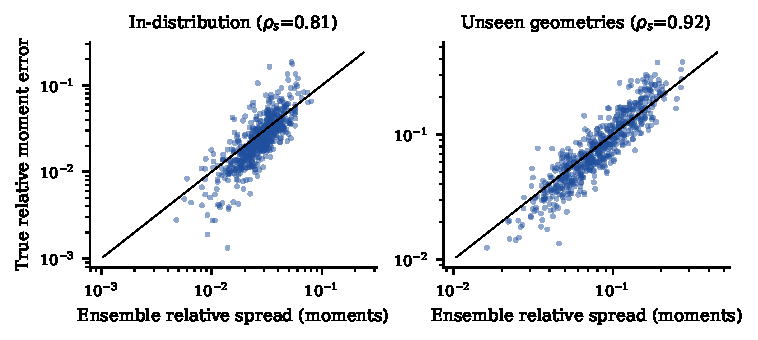
\includegraphics[width=\textwidth]{fig_uq_scatter.pdf}
\caption{Frame-level ensemble spread of the end moments $s$ (Eq.~\ref{eq:score}) against the true relative moment error for the four test sets. Black line: $e_M=s$; red dashed line: split-conformal bound $\hat a s$ calibrated on the validation frames.}\label{fig:uqscatter}
\end{figure}

The ensemble spread ranks the frames by their actual error well on in-distribution frames, on unseen geometries and on the design-driven frames (Spearman $\rho_s=0.81$, $0.92$ and $0.75$; Table~\ref{tab:uq} and Fig.~\ref{fig:uqscatter}), and the $\pm2\sigma$ intervals of the end moments contain 92\%, 92\% and 94\% of the PyNite values, close to the nominal 95\%. It is much weaker for unseen load patterns ($\rho_s=0.66$, coverage 67\%): the networks agree with each other on these frames while being wrong together, the known failure mode of ensembles under distribution shift~\cite{ovadia2019shift}. The label-free equilibrium residual of the raw prediction is a weaker indicator ($\rho_s=0.43$--$0.74$), which is why it is not used for referral.

\begin{table}[t]
\centering
\caption{Stage 1 of the referral rule: fraction of frames (\%) flagged as outside the training domain by the Mahalanobis distance of the frame descriptors, threshold at the 99th percentile of the validation frames.}\label{tab:ooddomain}
\footnotesize
\begin{tabular}{lrrrrr}
\toprule
Descriptors & Validation & ID & OOD-G & OOD-L & DES \\
\midrule
\inputtable{tables/tab_ood_domain.tex}
\bottomrule
\end{tabular}
\end{table}

The domain check (Table~\ref{tab:ooddomain}) flags 1.7\% of the ID test frames, close to the 1\% calibrated on the validation frames, and 79\% of the OOD-G and 75\% of the OOD-L frames. The two descriptor groups detect different shifts: the geometry descriptors flag 68\% of the unseen geometries but only 1.5\% of the unseen load patterns, and the load-pattern descriptors flag 67\% of the unseen load patterns but only 9\% of the unseen geometries. The load-pattern check therefore supplies exactly the information that the ensemble spread lacks. All 149 OOD-L frames that pass the check are frames whose random bay pattern happened to leave every bay fully loaded, so that only the lateral profile is new; the 129 OOD-G frames that pass are one step beyond the training range (45 have six storeys, 68 have five bays and at most five storeys). The check also flags 20\% of the design-driven frames, mainly because of their high gravity-to-lateral load ratio, their small roof share of the lateral load and their stiff material ($E$ at the upper end of the range), although the surrogate is accurate on all of them. The domain check is therefore conservative, which costs FE analyses but not accuracy.

\begin{table}[t]
\centering
\caption{Two-stage referral rule with thresholds fixed on the validation frames ($\hat a=1.41$ for $\alpha=0.1$). Referred: by the domain check, by the conformal bound $\hat a s>\tau$ and in total (\%). Coverage: share of in-domain frames with $e_M\le\hat a s$. Violation: share of accepted frames with $e_M>\tau$. p95: 95th percentile of $e_M$ over the accepted frames and over all frames (\%).}\label{tab:oodpolicy}
\footnotesize
\begin{adjustbox}{max width=\textwidth}
\begin{tabular}{llrrrrrrr}
\toprule
$\tau$ & Set & Domain & Bound & Total & Coverage & Violation & p95 accepted & p95 all \\
\midrule
\inputtable{tables/tab_ood_policy.tex}
\bottomrule
\end{tabular}
\end{adjustbox}
\end{table}

Table~\ref{tab:oodpolicy} evaluates the complete rule, whose two thresholds were fixed on the validation frames before the test sets were used. With a tolerance of $\tau=10\%$ on the relative moment error, the rule refers 2.2\% of the ID frames and accepts the rest with a violation rate of 1.4\% (frames whose true error exceeds 10\% although accepted). On unseen geometries it refers 86\% of the frames and the accepted 14\% have a 95th-percentile error of 7.7\% and a violation rate of 1.2\%, compared with a 95th percentile of 22.6\% and 35\% of frames above 10\% without referral. On unseen load patterns it refers 75\% and the accepted frames have a violation rate of 1.4\%. On the design-driven frames 20\% are referred by the domain check and none of the accepted frames exceeds 10\% (largest accepted error 4.8\%). With $\tau=5\%$ the violation rates are 3.5\% (ID), 17\% (OOD-G, 12 accepted frames), 5.4\% (OOD-L) and 0\% (DES), at the cost of referring 28\% of the ID frames. The conformal bound covers the true error in 90\% (ID), 94\% (OOD-G) and 99\% (DES) of the in-domain frames, matching the nominal 90\%, but only in 84\% of the in-domain OOD-L frames, so the coverage guarantee, which assumes exchangeability with the calibration frames, holds only approximately once the load pattern changes; the domain check is what keeps the accepted OOD-L frames safe. These numbers are the honest cost of the safety: the rule cannot make the surrogate accurate where it is not, but it makes the referral decision before the FE result is known and with thresholds that were not tuned on the test data.

\begin{figure}[p]
\centering
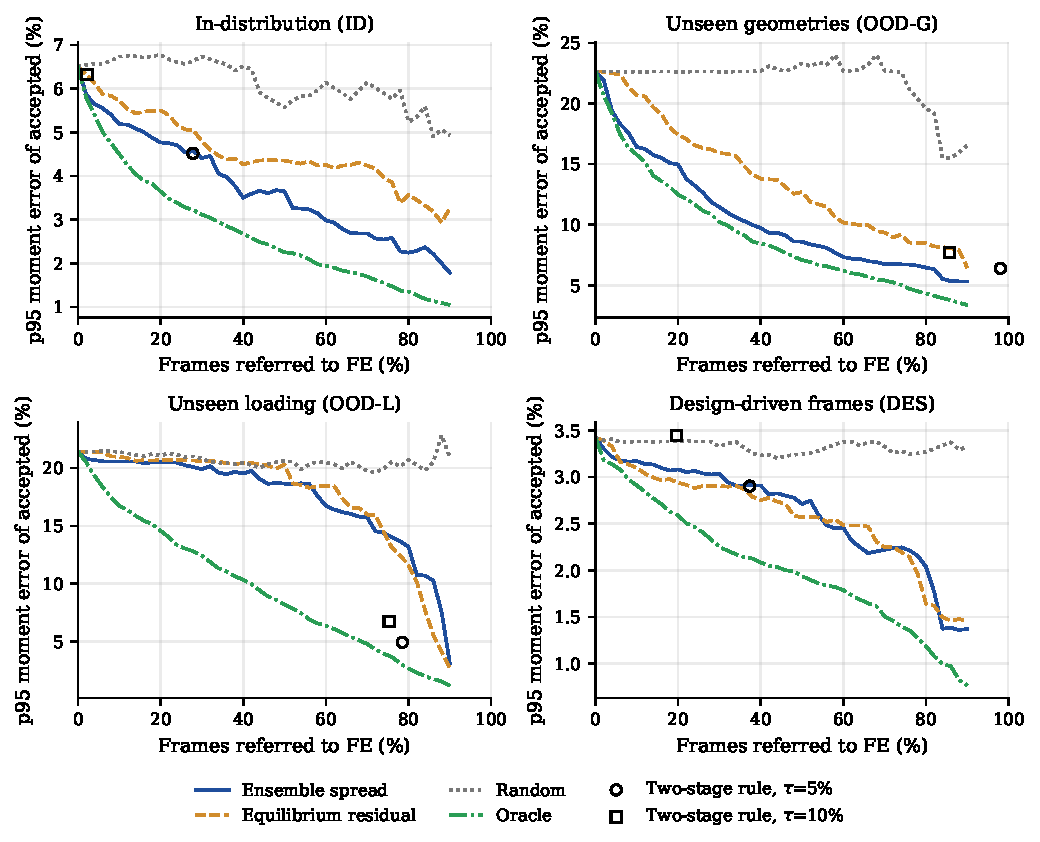
\includegraphics[width=\textwidth]{fig_triage.pdf}
\caption{Risk--coverage curves: 95th percentile of the moment error over the accepted predictions when the frames with the largest scores are referred to PyNite, for the ensemble spread, the equilibrium residual, random referral and an oracle ranking by the true error. Markers: operating points of the two-stage rule with validation-calibrated thresholds (Table~\ref{tab:oodpolicy}). The curves are computed on the test sets and serve only to describe the ranking quality.}\label{fig:triage}
\end{figure}

Figure~\ref{fig:triage} complements the rule with risk--coverage curves. On the ID set, referring the 20\% of frames with the largest spread lowers the 95th-percentile moment error from 6.5\% to 4.8\% and catches 78\% of the 1.5\% of frames with errors above 10\%. On unseen geometries it lowers the tail from 22.6\% to 15.0\%; on unseen load patterns the spread-based ranking is little better than random (21.4\%$\to$20.5\%), which is why the domain check is needed.
